\documentclass{article}

% if you need to pass options to natbib, use, e.g.:
% \PassOptionsToPackage{numbers, compress}{natbib}
% before loading nips_2016
%
% to avoid loading the natbib package, add option nonatbib:
% \usepackage[nonatbib]{nips_2016}

\usepackage[final]{nips_2016}

% to compile a camera-ready version, add the [final] option, e.g.:
% \usepackage[final]{nips_2016}

\usepackage[utf8]{inputenc} % allow utf-8 input
\usepackage[T1]{fontenc}    % use 8-bit T1 fonts
\usepackage{hyperref}       % hyperlinks
\usepackage{url}            % simple URL typesetting
\usepackage{booktabs}       % professional-quality tables
\usepackage{amsfonts}       % blackboard math symbols
\usepackage{nicefrac}       % compact symbols for 1/2, etc.
\usepackage{microtype}      % microtypography
\usepackage{graphicx}

\title{Report for the Deep Learning Course Assignment 2 }

% The \author macro works with any number of authors. There are two
% commands used to separate the names and addresses of multiple
% authors: \And and \AND.
%
% Using \And between authors leaves it to LaTeX to determine where to
% break the lines. Using \AND forces a line break at that point. So,
% if LaTeX puts 3 of 4 authors names on the first line, and the last
% on the second line, try using \AND instead of \And before the third
% author name.

\author{
  Georgios Methenitis \\
  \texttt{georgios.methenitis@cwi.nl}
}

\begin{document}
% \nipsfinalcopy is no longer used

\maketitle

\begin{abstract}
Should contain information about the current task and the summary of the study of the CNN models on CIFAR10 dataset.

\end{abstract}

\section{Task 1}
Should contain all needed information about Task 1 and report of all your experiments for that task.

Figure~\ref{fig:1}, \ref{fig:2}


\begin{figure}[h!]
\centering
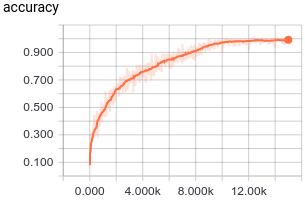
\includegraphics[height=3.2cm]{acc1.png}\	
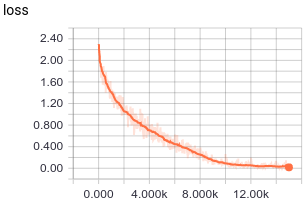
\includegraphics[height=3.2cm]{loss1.png}
\caption{Accuracy (left) and loss on the training set with batch size of $128$ samples. The accuracy approximates $1.0$ in the training set implying that the model overfits the training set.}
\label{fig:1}
\end{figure}


\begin{figure}[h!]
\centering
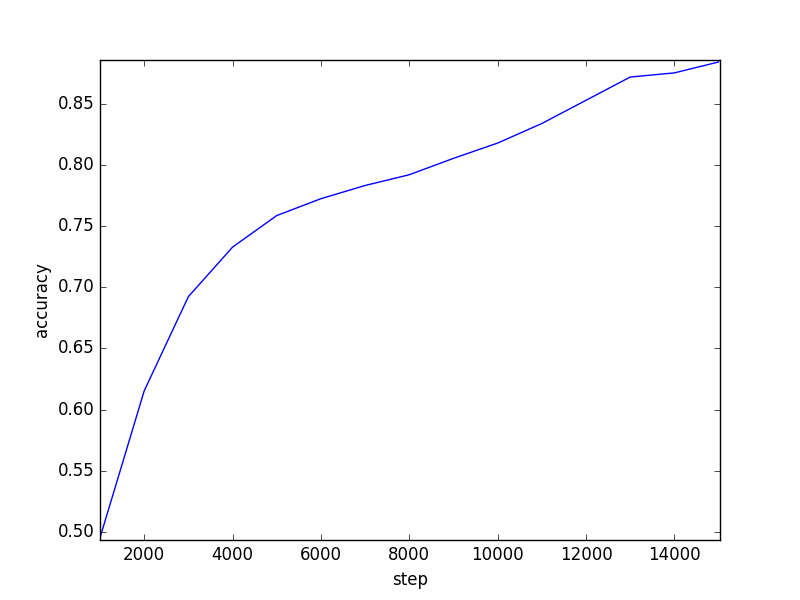
\includegraphics[height=3.2cm]{acc2.png}\	
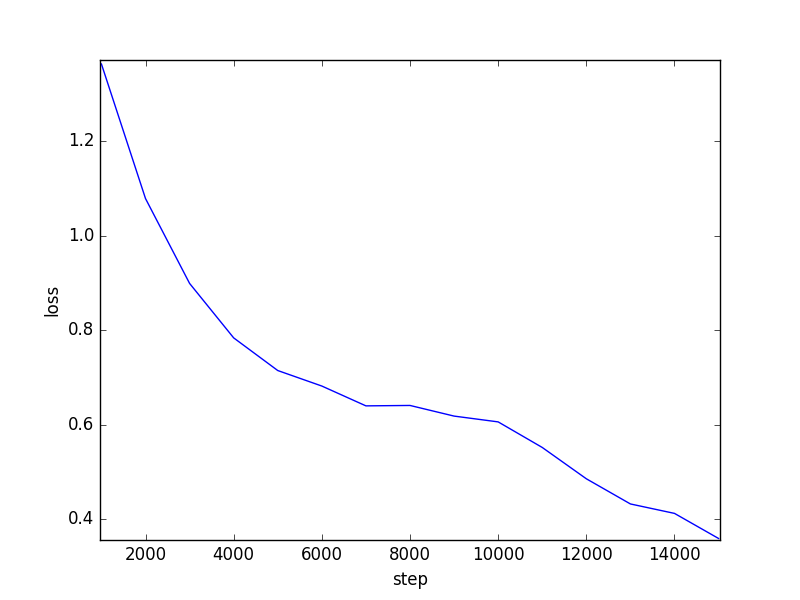
\includegraphics[height=3.2cm]{loss2.png}
\caption{Accuracy (left) and loss on the test set with batch size of $128$ samples. The accuracy is $0.88$ after $15000$ steps.}
\label{fig:2}
\end{figure}



\subsection{Smaller batch size}

Figure~\ref{fig:3}, \ref{fig:4}

\begin{figure}[h!]
\centering
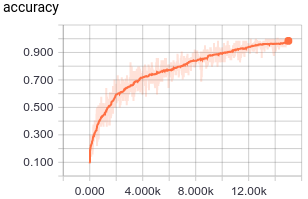
\includegraphics[height=3.2cm]{acc3.png}\	
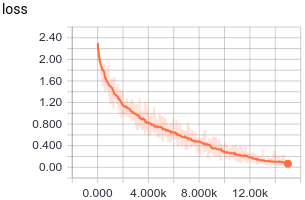
\includegraphics[height=3.2cm]{loss3.png}
\caption{Accuracy (left) and loss on the training set with batch size of $128$ samples. The accuracy approximates $1.0$ in the training set implying that the model overfits the training set.}
\label{fig:3}
\end{figure}


\begin{figure}[h!]
\centering
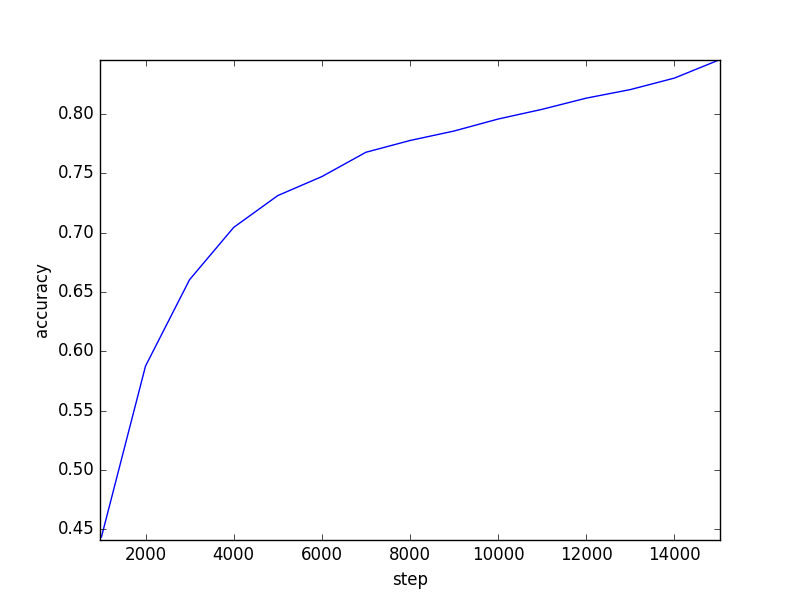
\includegraphics[height=3.2cm]{acc4.png}\	
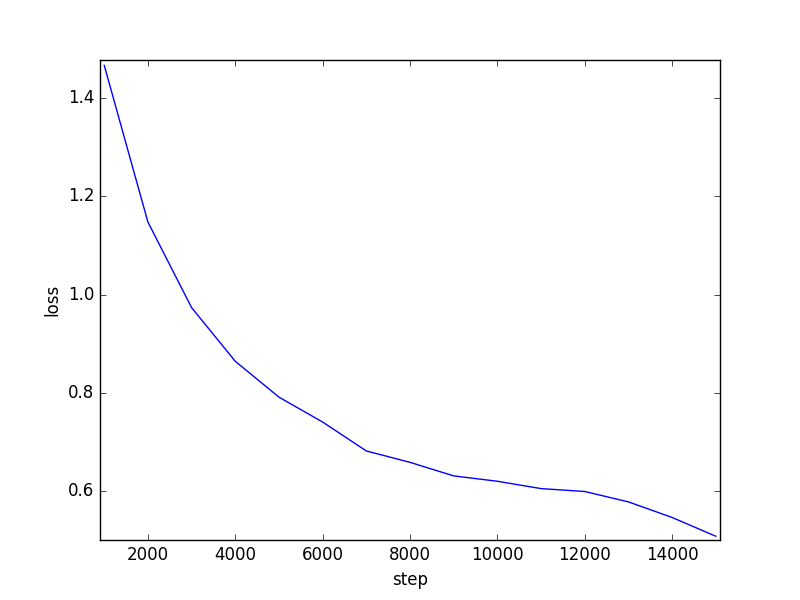
\includegraphics[height=3.2cm]{loss4.png}
\caption{Accuracy (left) and loss on the test set with batch size of $128$ samples. The accuracy is $0.88$ after $15000$ steps.}
\label{fig:4}
\end{figure}





\section{Task 2}
Should contain all needed information about Task 2 and report of all your experiments for that task.

\section{Task 3}
Should contain all needed information about Task 3 and report of all your experiments for that task.

\section{Conclusion}
Should contain conclusion of this study.

%\section*{References}
%
%\small
%
%[1] Alexander, J.A.\ \& Mozer, M.C.\ (1995) Template-based algorithms
%for connectionist rule extraction. In G.\ Tesauro, D.S.\ Touretzky and
%T.K.\ Leen (eds.), {\it Advances in Neural Information Processing
%  Systems 7}, pp.\ 609--616. Cambridge, MA: MIT Press.
%
%[2] Bower, J.M.\ \& Beeman, D.\ (1995) {\it The Book of GENESIS:
%  Exploring Realistic Neural Models with the GEneral NEural SImulation
%  System.}  New York: TELOS/Springer--Verlag.
%
%[3] Hasselmo, M.E., Schnell, E.\ \& Barkai, E.\ (1995) Dynamics of
%learning and recall at excitatory recurrent synapses and cholinergic
%modulation in rat hippocampal region CA3. {\it Journal of
%  Neuroscience} {\bf 15}(7):5249-5262.

\end{document}
